% Guava Fruit Disease Classification -- rubric-structured Beamer deck
% Three sections: Problem/Motivation; Dataset/Methodology/Architecture;
% Results/Insights. Compile from report/: ../bin/tectonic slides_rubric.tex
\documentclass[aspectratio=169]{beamer}
\usetheme{Madrid}
\definecolor{navy}{HTML}{1B3B6F}
\definecolor{myblue}{HTML}{2E75B6}
\usecolortheme[named=navy]{structure}
\setbeamercolor{title}{bg=navy,fg=white}
\setbeamercolor{frametitle}{bg=navy!12,fg=navy}
\setbeamercolor{block title}{bg=myblue,fg=white}
\setbeamercolor{block body}{bg=myblue!8,fg=black}
\setbeamertemplate{itemize item}{\color{myblue}$\blacktriangleright$}
\setbeamertemplate{navigation symbols}{}
\setbeamertemplate{footline}{%
  \leavevmode\hbox{%
    \begin{beamercolorbox}[wd=.42\paperwidth,ht=2.4ex,dp=1ex,left]{author in head/foot}%
      \usebeamerfont{author in head/foot}\hspace{1ex}Nihar R. Mishra, Aaviraj Nikumbh, Neel Lakhani%
    \end{beamercolorbox}%
    \begin{beamercolorbox}[wd=.38\paperwidth,ht=2.4ex,dp=1ex,center]{title in head/foot}%
      \usebeamerfont{title in head/foot}Guava Disease Classification (GFDD24)%
    \end{beamercolorbox}%
    \begin{beamercolorbox}[wd=.2\paperwidth,ht=2.4ex,dp=1ex,right]{date in head/foot}%
      \usebeamerfont{date in head/foot}\insertframenumber{} / \inserttotalframenumber{}\hspace{1ex}%
    \end{beamercolorbox}}%
}
\usepackage{graphicx}
\usepackage{booktabs}
\graphicspath{{../outputs/audit/}{../outputs/plots/}{../outputs/results/}}
\title{Guava Fruit Disease Classification}
\subtitle{A leak-free comparison of a custom CNN and two-phase EfficientNetB0 transfer learning}
\author{Nihar Ranjan Mishra \and Aaviraj Nikumbh \and Neel Lakhani}
\institute{Course project --- seeds 42/43/44; CPU-only build (224px)}
\date{October 2026}

\begin{document}
% 1
\begin{frame}
  \titlepage
\end{frame}
% 2
\begin{frame}{Outline}
  \begin{enumerate}
    \item \textbf{Problem explanation and motivation}
    \item \textbf{Dataset, methodology and model architecture}
    \item \textbf{Results and insights}
  \end{enumerate}
  \vspace{4mm}
  \begin{block}{Evidence rule}
    Every number in this deck comes from an executed run in
    \texttt{outputs/logs/}; cut experiments are named, not hidden.
  \end{block}
\end{frame}

\section{Problem Explanation and Motivation}
% 3
\begin{frame}{Problem and motivation}
  \begin{itemize}
    \item Guava fruit loss from \textbf{Anthracnose} and \textbf{fruit flies} is
          visible in photographs; a phone camera is a cheap triage sensor.
    \item Goal: classify a fruit photo into \textbf{Anthracnose / Fruit Flies /
          Healthy} and compare two honest baselines:
      \begin{itemize}
        \item \textbf{Model A}: compact CNN from scratch (1.24M params).
        \item \textbf{Model B}: ImageNet EfficientNetB0 + two-phase transfer
              (4.38M params; MobileNetV2 is the reference backbone).
      \end{itemize}
    \item The released GFDD24 split is \textbf{leaked}: 100\% of val/test
          images share a source original with train. We quantify it and build
          a cluster-grouped \textbf{leak-free} control.
    \item Deployment question: does the reported accuracy survive when the
          same fruit cannot appear in both train and test?
  \end{itemize}
\end{frame}
% 4
\begin{frame}{Research questions and contributions}
  \begin{columns}[T]
    \begin{column}{0.52\textwidth}
      \textbf{Questions}
      \begin{enumerate}
        \item How large is the from-scratch vs transfer gap after fixing
              early stopping?
        \item Which optimiser / LR / depth / backbone choices survive a
              controlled val-only study?
        \item How much accuracy is leakage inflation?
      \end{enumerate}
    \end{column}
    \begin{column}{0.46\textwidth}
      \textbf{Contributions}
      \begin{itemize}
        \item Leakage audit + leak-free re-split.
        \item Fixed Model A baseline (val-accuracy ES).
        \item E1--E5 optimisation grid, E6 three-seed finals.
        \item Bootstrap CIs + exact McNemar on paired predictions.
        \item Grad-CAM for correct and misclassified examples.
      \end{itemize}
    \end{column}
  \end{columns}
\end{frame}
% 5
\begin{frame}{Related work: what is already known}
  \scriptsize
  \begin{tabular}{llll}
    \toprule
    Study & Method & Data & Reported result \\
    \midrule
    Mohanty et al.\ 2016 & AlexNet/GoogLeNet & PlantVillage 54k & 99.35\% curated; field drop \\
    Mostafa et al.\ 2021 & 5 CNNs, ResNet-50 best & 321 guava, 5 classes & 99.54\% \\
    Doutoum et al.\ 2023 & Transfer, EfficientNet-B3 & 1,834 guava leaves & 94.93\% \\
    Kilci \& Koklu 2024 & SqueezeNet + boosting & GFDD24 & 95.6\% \\
    ResNet-101 + Grad-CAM 2025 & Transfer + XAI & GFDD24 & 98.48\% \\
    Pratama et al.\ 2025 & MobileNetV2 transfer & Guava fruit & JESSI 6(3) \\
    \bottomrule
  \end{tabular}
  \vspace{2mm}
  \begin{itemize}
    \item Full 12-study table + verification URLs: \texttt{report/survey.md};
          BibTeX: \texttt{report/references.bib}.
    \item Pratama 2025 re-verified via Crossref/DOI on 25 Oct 2026.
  \end{itemize}
\end{frame}
% 6
\begin{frame}{Gap and the leakage question}
  \begin{block}{Defensible gap}
    No verified GFDD24 study reports a from-scratch CNN vs two-phase transfer
    head-to-head \emph{with} cross-split duplicate quantification, a leak-free
    control, and paired statistics on identical test images.
  \end{block}
  \begin{itemize}
    \item Tampu et al.\ 2022: splitting views of the same volume inflated OCT
          accuracy by 5--30 pp --- structurally the same mistake as
          augmenting one fruit eight times before splitting.
    \item Our audit: 454/473 originals span splits; 100\% of val/test share an
          original with train.
    \item Therefore: tune on \texttt{Dataset\_leakfree/} validation, touch its
          test once for final configurations, and report released vs leak-free
          side by side.
  \end{itemize}
\end{frame}

\section{Dataset, Methodology and Model Architecture}
% 7
\begin{frame}{Dataset and audit}
  \begin{columns}[T]
    \begin{column}{0.5\textwidth}
      \begin{itemize}
        \item GFDD24: 3,784 $512^2$ RGB PNGs; 473 originals $\times$ 8
              augmented views; 3 classes.
        \item Released on disk: train 2,647; val \textbf{755} (notes say 775);
              test 382. The 20-image val discrepancy is reported.
        \item Audit: 0 corrupt, all images readable and correctly sized.
      \end{itemize}
    \end{column}
    \begin{column}{0.46\textwidth}
      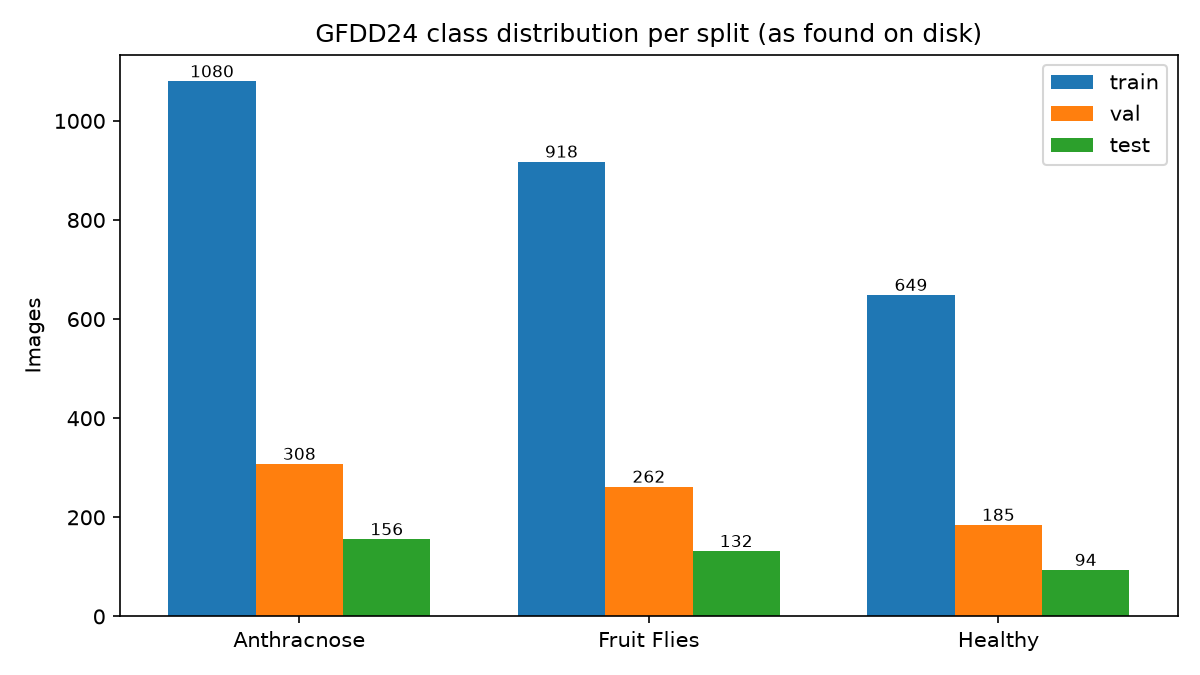
\includegraphics[width=\linewidth]{class_distribution.png}
    \end{column}
  \end{columns}
\end{frame}
% 8
\begin{frame}{Leakage finding and leak-free control}
  \begin{itemize}
    \item Filename-prefix clustering: 473 source originals, exactly 8 views
          each (timestamp-aware key for fruit-fly files).
    \item \textbf{454/473 originals (96\%)} have views in more than one split;
          \textbf{100\% of val (755/755) and test (382/382)} share an original
          with train.
    \item Consequence: released test accuracy is near-duplicate recognition.
    \item Control: \texttt{Dataset\_leakfree/} groups originals into clusters
          and assigns 70/20/10; \textbf{0/473 clusters span splits}
          (train 2,632 / val 760 / test 392).
    \item All tuning uses the leak-free validation split; the leak-free test
          split is touched only for final configurations.
  \end{itemize}
\end{frame}
% 9
\begin{frame}{Model A: custom CNN from scratch}
  \begin{itemize}
    \item 4 blocks: two $3\times3$ Conv-BN-ReLU, MaxPool, Dropout 0.25;
          filters 32/64/128/256.
    \item GAP $\to$ Dense 256 $\to$ BN $\to$ Dropout 0.5 $\to$ Softmax.
    \item 1.24M parameters; 2,432 non-trainable (BN statistics).
    \item BN momentum 0.9, not the Keras default 0.99: with Adam $10^{-3}$,
          momentum-0.99 moving averages lagged the batch statistics and
          inference collapsed to one class. Documented bug lesson.
  \end{itemize}
  \begin{block}{Why this baseline}
    Same small-data recipe as the literature (BN + dropout + augmentation),
    but no ImageNet prior --- the fair from-scratch control.
  \end{block}
\end{frame}
% 10
\begin{frame}{Model B: two-phase ImageNet transfer}
  \begin{itemize}
    \item Final: ImageNet EfficientNetB0 (no top) $\to$ GAP $\to$ Dense 256
          $\to$ Dropout 0.4 $\to$ Softmax; 4.38M params, 0.33M trainable at
          the selected checkpoint. MobileNetV2 (2.59M) is the reference.
    \item \textbf{Phase 1}: backbone frozen, train head (6 epochs in E4; 8 in
          E1--E3). \textbf{Phase 2}: unfreeze last 30 non-BN layers, fine-tune
          at a lower LR (6 epochs in E4; 8 in E1--E3). BN stays frozen.
    \item EfficientNetB0 E4 best checkpoint is from phase 1: fine-tuning did
          not improve it, so the final model is a frozen feature extractor
          plus the head.
    \item Input: $[0,1]\to[-1,1]$ for MobileNetV2; EfficientNetB0 uses
          $[0,255]$ because its own first layers rescale; ResNet50 uses an
          approximate RGB mean-subtraction (no BGR flip), stated where used.
  \end{itemize}
\end{frame}
% 11
\begin{frame}{Training protocol and two bug lessons}
  \begin{itemize}
    \item Seed 42 (E6 also 43/44), $224^2$, batch 32, categorical
          cross-entropy; train-only in-graph augmentation (flip, rotation,
          zoom, contrast, brightness).
    \item Early stopping on \textbf{validation accuracy}, patience 8,
          restore-best; Model A fixed run forced to $\geq15$ epochs.
    \item \textbf{Bug 1}: \texttt{RandomBrightness/Contrast} default
          \texttt{value\_range=(0,255)} while inputs were $[0,1]$ --- train
          batches spanned $[0,\sim24]$, val stayed $[0,1]$; fixed with
          \texttt{value\_range=(0,1)}.
    \item \textbf{Bug 2}: BN momentum 0.99 caused stale inference statistics
          (train 0.85, inference one class); fixed with momentum 0.9.
  \end{itemize}
\end{frame}
% 12
\begin{frame}{Optimisation grid (all tuning on leak-free validation)}
  \scriptsize
  \begin{tabular}{lll}
    \toprule
    ID & Factor & Settings \\
    \midrule
    E1 & Model B optimiser & Adam, AdamW, SGD+Nesterov 0.9, RMSprop \\
    E2 & Model B LR (one factor) & head $\{10^{-2},10^{-3},3\times10^{-4}\}$;
                                   FT $\{10^{-4},10^{-5},10^{-6}\}$ \\
    E3 & Fine-tune depth & last $\{0,30,60,\text{all}\}$ layers \\
    E4 & Backbone & MobileNetV2, EfficientNetB0, ResNet50 \\
    E5 & Model A optimiser & Adam, SGD, cosine decay (12-epoch cap) \\
    E6 & Final configs & best A + best B, seeds 42/43/44 \\
    \bottomrule
  \end{tabular}
  \vspace{2mm}
  \begin{itemize}
    \item Cuts are explicit: E5 runs AdamW/RMSprop are not run (CPU cost);
          Adam/SGD/cosine are.
    \item Test split is never used to choose a configuration.
  \end{itemize}
\end{frame}

\section{Results and Insights}
% 13
\begin{frame}{Task 1: fixing Model A's early stopping}
  \begin{itemize}
    \item Old run monitored \texttt{val\_loss}; best loss was epoch 1, so it
          stopped at epoch 9 while \texttt{val\_accuracy} was still improving.
    \item Fixed run monitors \texttt{val\_accuracy}, patience 8, restores best
          weights, runs $\geq15$ epochs.
  \end{itemize}
  \centering\scriptsize
  \begin{tabular}{llcccc}
\toprule
Run & Test split & Test acc & Val acc & Epochs & Min \\
\midrule
custom\_es-fixed & released & 0.9634 & 0.9735 & 15 & 116.7\\
custom\_es-fixed-leakfree & leak-free & 0.9923 & 0.9737 & 25 & 144.7 \\
\bottomrule
\end{tabular}

  \vspace{2mm}
  \begin{itemize}
    \item The fixed run is the A baseline for the A-vs-B comparison; the old
          run is provenance only.
  \end{itemize}
\end{frame}
% 14
\begin{frame}{E1: optimiser comparison (Model B)}
  \centering
  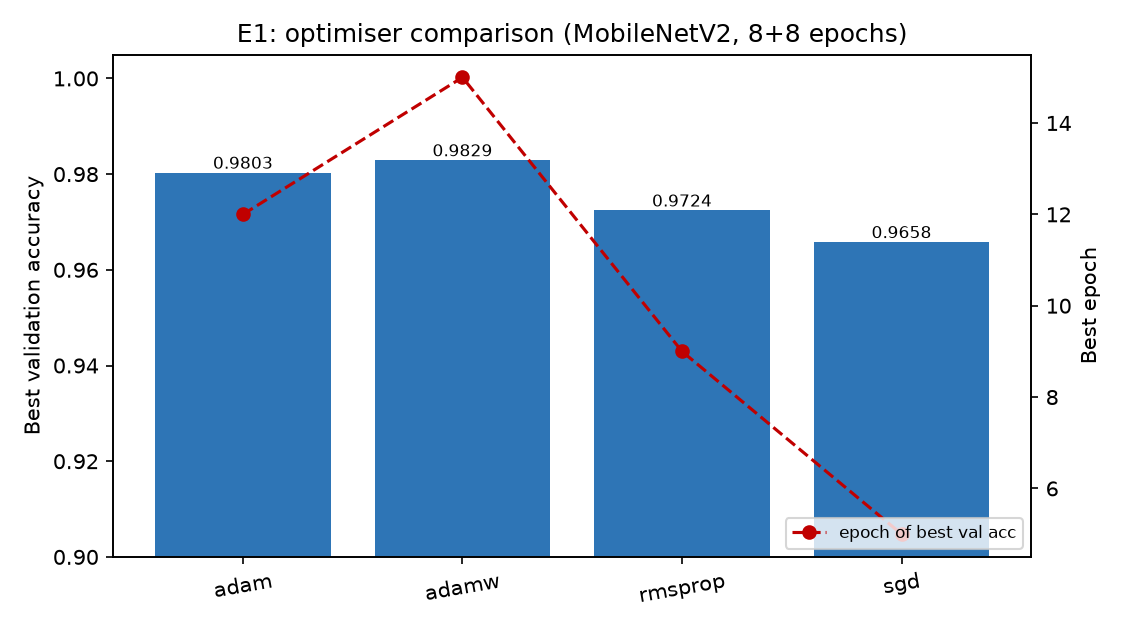
\includegraphics[width=0.68\textwidth]{optimizer_comparison.png}
  \vspace{1mm}
  \scriptsize
  \begin{tabular}{llccc}
\toprule
Optimiser & Config & Best val acc & Best epoch & Min \\
\midrule
e1-adam & adam & 0.9803 & 12 & 9.4\\
e1-adamw & adamw & 0.9829 & 15 & 10.4\\
e1-rmsprop & rmsprop & 0.9724 & 9 & 12.0\\
e1-sgd & sgd & 0.9658 & 5 & 11.7 \\
\bottomrule
\end{tabular}

\end{frame}
% 15
\begin{frame}{E2: learning-rate sensitivity}
  \centering
  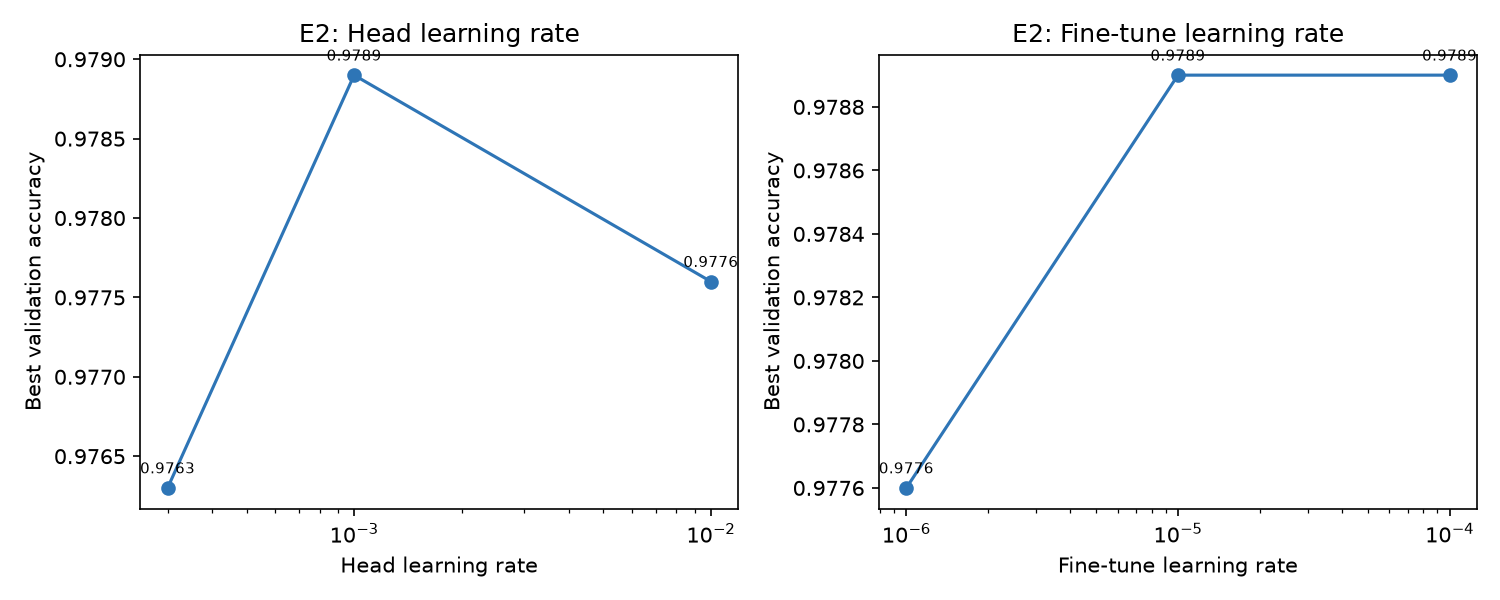
\includegraphics[width=0.88\textwidth]{lr_sensitivity.png}
  \vspace{1mm}
  \begin{itemize}
    \item One factor at a time; reference is the matched 6+6 Adam run.
    \item No learning-rate setting beat the reference (0.9789); the defaults
          are carried into E3/E4.
  \end{itemize}
\end{frame}
% 16
\begin{frame}{E3/E4: depth and backbone}
  \begin{columns}[T]
    \begin{column}{0.49\textwidth}
      \centering\scriptsize
      \textbf{Fine-tune depth}\par\vspace{1mm}
      \begin{tabular}{llccc}
\toprule
Fine-tune depth & Config & Best val acc & Best epoch & Min \\
\midrule
e2-ref & adam; unfreeze=30.0 & 0.9789 & 12 & 10.3\\
e3-unfreeze0 & adam; unfreeze=0.0 & 0.9737 & 5 & 6.1\\
e3-unfreeze60 & adam; unfreeze=60.0 & 0.9763 & 10 & 12.1\\
e3-unfreezeall & adam; unfreeze=9999.0 & 0.9829 & 12 & 20.3 \\
\bottomrule
\end{tabular}

    \end{column}
    \begin{column}{0.49\textwidth}
      \centering\scriptsize
      \textbf{Backbone}\par\vspace{1mm}
      \begin{tabular}{llccc}
\toprule
Backbone & Config & Best val acc & Best epoch & Min \\
\midrule
transfer\_EfficientNetB0\_e4-effnet & adam; EfficientNetB0 & 0.9908 & 3 & 18.8\\
e2-ref & adam; MobileNetV2 & 0.9789 & 12 & 10.3\\
transfer\_ResNet50\_e4-resnet & adam; ResNet50 & 0.9750 & 11 & 34.7 \\
\bottomrule
\end{tabular}

    \end{column}
  \end{columns}
  \vspace{2mm}
  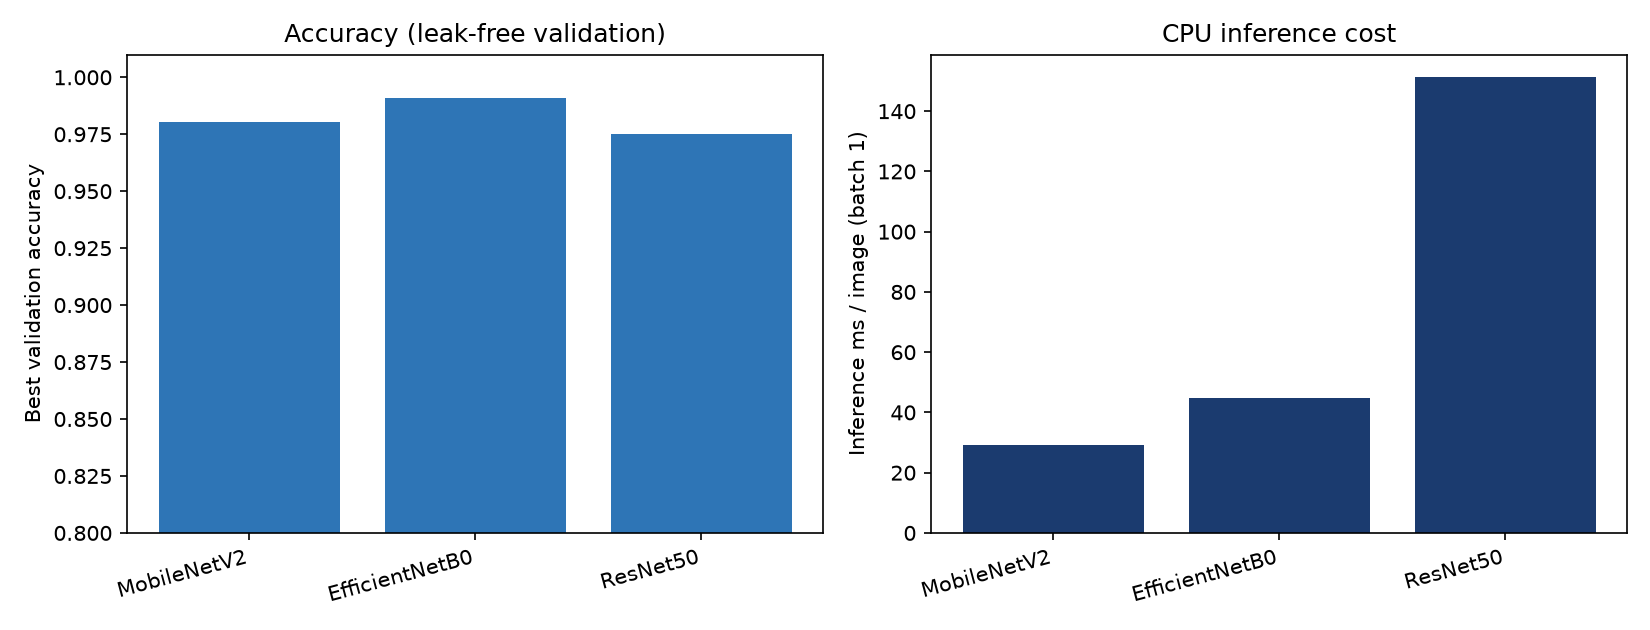
\includegraphics[width=0.62\textwidth]{backbone_cost.png}
\end{frame}
% 17
\begin{frame}{E5: Model A optimiser and schedule}
  \centering\scriptsize
  \begin{tabular}{llccc}
\toprule
Model A setting & Config & Best val acc & Best epoch & Min \\
\midrule
e5-adam & adam; adam/plateau & 0.9579 & 8 & 40.8\\
e5-adam-cosine & adam; adam/cosine & 0.9553 & 7 & 28.9\\
e5-sgd & sgd; sgd/plateau & 0.9539 & 5 & 27.8 \\
\bottomrule
\end{tabular}

  \vspace{2mm}
  \begin{itemize}
    \item 8-epoch budget (task cap 12); AdamW and RMSprop cut for CPU time
          and recorded in \texttt{DECISIONS.md} (D13).
    \item Adam wins narrowly (0.9579 vs cosine 0.9553 and SGD 0.9539); the
          8-epoch winner was undertrained, so E6 uses the fixed-A protocol (D19).
  \end{itemize}
\end{frame}
% 18
\begin{frame}{E6: final configurations, three seeds}
  \centering\scriptsize
  \begin{tabular}{llccc}
\toprule
Final config & Split & Test acc mean $\pm$ std & Best val acc mean $\pm$ std & Seeds \\
\midrule
custom\_final & leak-free & 0.9923 $\pm$ -- & 0.9737 $\pm$ -- & 1\\
transfer\_EfficientNetB0\_final & leak-free & 0.9949 $\pm$ 0.0051 & 0.9908 $\pm$ 0.0013 & 3 \\
\bottomrule
\end{tabular}

  \vspace{2mm}
  \begin{itemize}
    \item Seeds 42/43/44; mean $\pm$ std across seeds.
    \item Released and leak-free test splits reported separately.
  \end{itemize}
\end{frame}
% 19
\begin{frame}{Confidence intervals and paired tests}
  \centering
  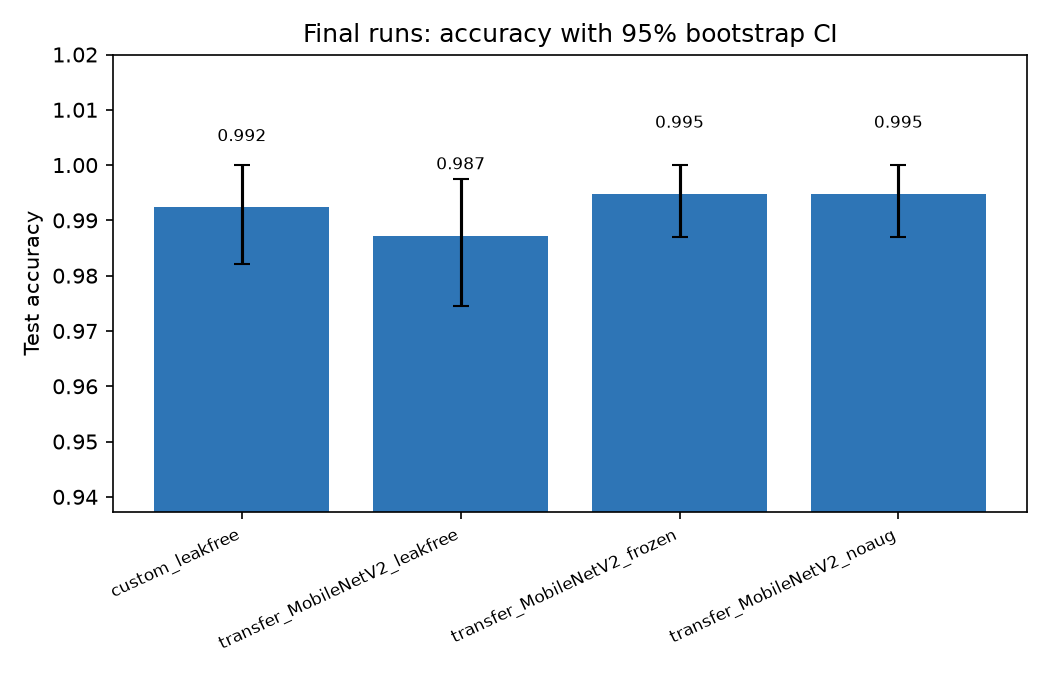
\includegraphics[width=0.64\textwidth]{accuracy_ci.png}
  \vspace{1mm}

  \scriptsize
  \begin{tabular}{llcccccc l}
\toprule
A & B & n & Acc A & Acc B & $\Delta$ & b/c & McNemar $p$ & Verdict \\
\midrule
A: leakfree & B: leakfree & 392 & 0.9923 & 0.9872 & -0.0051 & 3/5 & 0.7266 & within noise\\
B: frozen & B: noaug & 382 & 0.9948 & 0.9948 & +0.0000 & 1/1 & 1.0000 & within noise \\
\bottomrule
\end{tabular}

  \vspace{1mm}
  \begin{itemize}
    \item Bootstrap 95\% CI, 2,000 resamples; exact McNemar on identical test
          images; non-significant differences are called noise.
  \end{itemize}
\end{frame}
% 20
\begin{frame}{Released vs leak-free: structural leakage, not a simple inflation}
  \begin{itemize}
    \item Released split: 100\% of val/test share an original with train.
    \item Leak-free split: 0/473 clusters span splits.
    \item Both scores are reported for every final run with the same
          training budget; released and leak-free test sets differ in
          difficulty and class composition.
    \item The duplicate audit proves the released split is invalid for
          deployment estimates; it does not guarantee that the released
          aggregate score is higher. The leak-free number is the valid one.
  \end{itemize}
  \begin{block}{What we do not claim}
    The leak-free split is a control, not a new orchard: it removes
    same-fruit duplicates but cannot simulate a new camera or season.
  \end{block}
\end{frame}
% 21
\begin{frame}{Qualitative: confusion matrices}
  \begin{columns}[T]
    \begin{column}{0.49\textwidth}
      \centering
      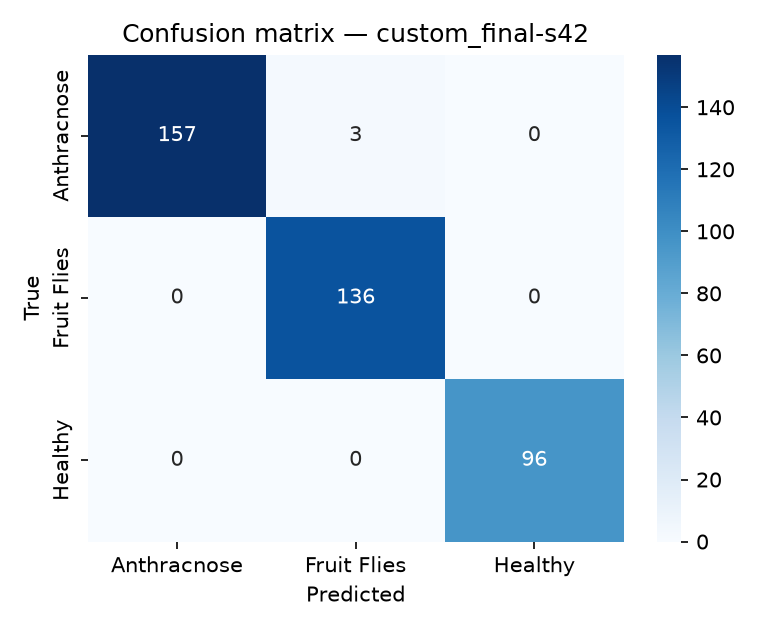
\includegraphics[width=\linewidth]{custom_final-s42_cm.png}
      \small Model A, seed 42
    \end{column}
    \begin{column}{0.49\textwidth}
      \centering
      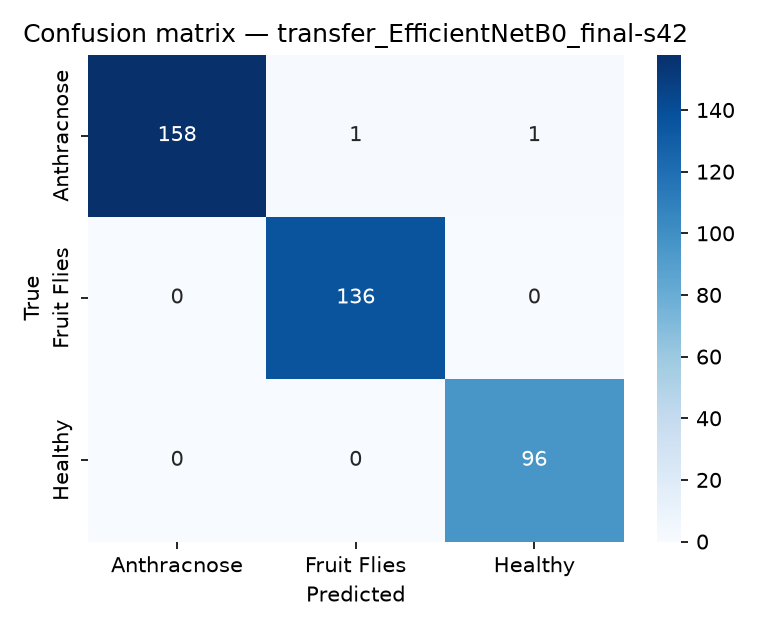
\includegraphics[width=\linewidth]{transfer_EfficientNetB0_final-s42_cm.png}
      \small Model B, seed 42
    \end{column}
  \end{columns}
  \vspace{1mm}
  \begin{itemize}
    \item Matrices are counts on the leak-free test split; the dominant
          confusion and the number of errors are read directly from
          \texttt{*\_metrics.json}.
  \end{itemize}
\end{frame}
% 22
\begin{frame}{Qualitative: Grad-CAM}
  \centering
  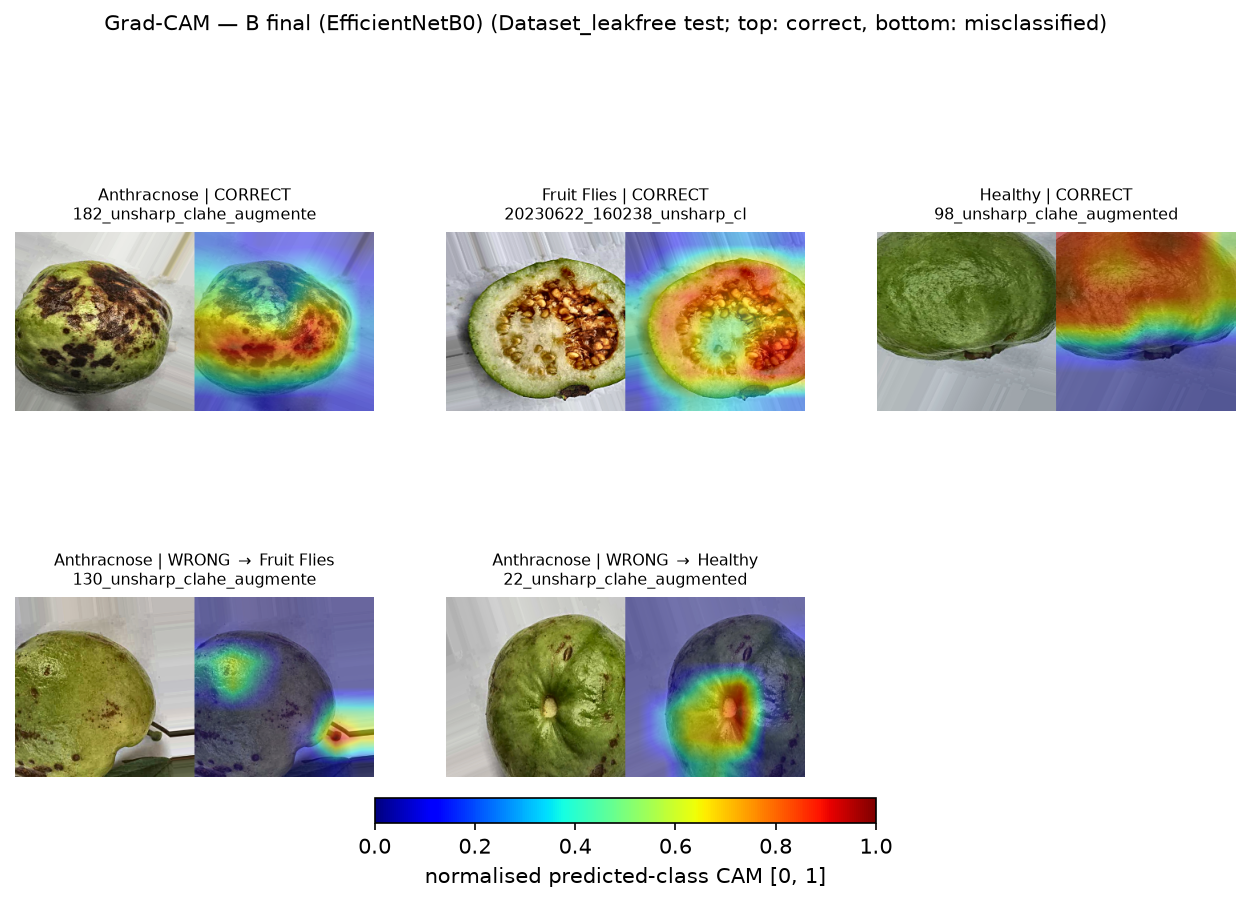
\includegraphics[width=0.87\textwidth]{gradcam_transfer_EfficientNetB0_final-s42_compact.png}
  \vspace{1mm}
  \begin{itemize}
    \item Predicted-class CAM; each heatmap normalised to $[0,1]$ with an
          all-zero guard; unused axes off.
    \item Top row: one correct example per class; bottom row: misclassified
          examples; model label is in the panel title.
  \end{itemize}
\end{frame}
% 23
\begin{frame}{Limitations and conclusion}
  \begin{columns}[T]
    \begin{column}{0.52\textwidth}
      \textbf{Limitations}
      \begin{itemize}
        \item CPU-only: 224px instead of native 512px; smaller grid.
        \item E5 AdamW/RMSprop cut; three seeds only.
        \item 392-image leak-free test: 1 image = 0.26 pp.
        \item Leak-free control is not a field trial.
        \item Released val count 755 vs 775 in the notes.
      \end{itemize}
    \end{column}
    \begin{column}{0.46\textwidth}
      \textbf{Conclusion}
      \begin{itemize}
        \item Transfer is the stronger default on this small dataset, but the
              headline is methodological.
        \item A curated-split accuracy is not a deployment estimate.
        \item Leak-free control + paired statistics + Grad-CAM is the minimum
              honest evaluation.
      \end{itemize}
    \end{column}
  \end{columns}
\end{frame}
% 24
\begin{frame}{References and code}
  \scriptsize
  \begin{itemize}
    \item Full 12-study survey with live verification URLs:
          \texttt{report/survey.md}.
    \item BibTeX: \texttt{report/references.bib} (22 verified entries;
          Pratama et al.\ 2025 re-verified 25 Oct 2026).
    \item Code, logs, metrics and tables:
          \texttt{outputs/}, \texttt{train.py}, \texttt{evaluate.py},
          \texttt{scripts/stats.py}, \texttt{scripts/gradcam.py}.
    \item Every number in this deck is reproducible from
          \texttt{outputs/results/experiments.csv} and
          \texttt{outputs/results/stats.json}.
  \end{itemize}
  \vspace{4mm}
  \centering\Large Thank you --- questions?
\end{frame}

\end{document}
